% compiling and viewing latex in os x
% brew cask install mactex
% /Library/TeX/texbin/pdflatex main.tex 

\documentclass{article}
\usepackage[T1]{fontenc}
\usepackage[utf8]{inputenc}
% \usepackage{lmodern}


\usepackage{listings}
\usepackage{float}
\title{Hootcoin de-centralized uncensorable open source distributed computing, live streaming Protocol and Marketplace Technical Whitepaper}
\author{Hootcoin Protocol Team}
\date{July 26 2017}
\setlength{\parskip}{1em}
\usepackage{natbib}
\usepackage{graphicx}
\usepackage{amssymb}
\usepackage{amsmath}
\usepackage{nameref}
\usepackage[normalem]{ulem}
% \usepackage{soul}
\usepackage[table]{xcolor}
\usepackage{tabularx}
\usepackage[english, status=draft]{fixme}
\fxusetheme{color}

\begin{document}

\maketitle

\begin{abstract}
The Hootcoin team is building the next generation technology for live
Streaming and distributed computing services based on blockchain technology and a new
innovative open source de-centralized live streaming and distributed computing protocol that would completely eliminate expensive content delivery networks and use peer-to-peer nodes for delivering not just live streaming video but also archived videos. This can be generalized to build a web scale cryptographically secure distributed computing environment creating the worlds first IPCN - interplanetary compute network.

A peer-to-peer hyperstream protocol to make the live streaming faster, safer, and completely open.

\sout{We will use crypto-financing (Initial Coin Offering) for capital rather than traditional venture capital and shareholders.}

\end{abstract}
\newpage

\tableofcontents
\newpage

\section{Introduction}
\subsection{History of Live Streaming}
Over the last half a century, people have been fascinated by live video. On September 4, 1951, Harry Truman spoke at the Japanese Peace Treaty Conference in San Francisco and, this was the worlds first live broadcast. Four months later, The Today Show would become the first broadcast news program airing live in the United States. Since then, we have loved live video, from our favorite news stations to our guilty pleasures of reality television.

\sout{Streaming is a lot older in its origins than one might intuitively suppose. One of the earliest streaming platforms was Muzak. This along with similar audio systems played continuous music. When we think of streaming, though, we think computers and the Internet. The full development of that capacity was more recent. Many technical advances in the 1990s and 2000s improved the bandwidth of networks. This increased the number of people and computers with access to those networks, creating the Internet as we know it today. Standard formats were also developed and protocols that we use to code online material and functions (TCP/IP, HTTP, HTML, etc.).}

As the bandwidth of connections to the Internet and computing power available to the average person continued to increase, it was natural that the audio streaming used by Internet radio would graduate to streaming video. Data compression methods contributed a lot to this development as well. Video files contain a lot of information. Compression allows that information to be efficiently transmitted and stored.

\subsection{Live Streaming versus On-Demand Streaming}
The term “live streaming” is sometimes applied where it doesn’t belong. Streaming from a recorded source, which is what one finds on YouTube, Netflix, and many other commercial streaming sources, is on-demand streaming. This means that the user can watch the content at will, while live streaming occurs only at the moment, in real-time. Live streaming comes from a content source such as video cameras and microphones. It is made available at the same time as the event being filmed occurs. On-demand streaming provides content from a recorded source instead. Streaming radio and much Internet television consists of live streaming.
As far as the “streaming” portion of the process is concerned, live and on-demand streaming are similar from the viewer’s perspective. They are quite different in technical and procedural details from the standpoint of the producer or broadcaster, though. The main difference from a technical end is the use of temporary storage for the material in progressive streaming or on-demand streaming. This is where a file is partially downloaded, stored to memory, and played while the next portion of the file is downloading. True streaming or live streaming doesn’t employ partial memory capture. It streams directly from the source to the user via a computer processor that finalizes the broadcast.

\section{Blockstack, Toshi, Status and the august beginnings of de-centralized
  web revolution}
  The internet is in the middle of a decentralization revolution: centralized proprietary services are being replaced with decentralized open ones with open source code; trusted parties replaced with verifiable mathematical computation; brittle location addresses replaced with resilient content addresses; inefficient monolithic services replaced with peer-to-peer algo- rithmic markets. Bitcoin, Ethereum, and other blockchain networks have proven the utility of decentralized transaction ledgers. These public ledgers process sophisticated smart contract applications and transact crypto-assets worth tens of billions of dollars every day. These systems are the first instances of internet-wide Open Services, where participants form a decentralized network providing useful services for pay, with no central management or trusted parties.
  
% \textbf{Netscape moment}: \emph{Cambrian} explosion of crypto-currency Ðapps
 
% \newcolumntype{Y}{>{\centering\arraybackslash}X}

 \begin{adjustbox}{width=.75\textwidth}
\begin{tabularx} {\textwidth}{|X|X|X|X|}
 \hline
& 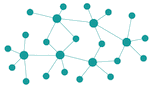
\includegraphics[scale=0.2]{static/decentnew} & 
\includegraphics[scale=0.2]{static/hootcoin} & \\
 \hline
\textbf{Phase} & \textbf{Internet} & \textbf{Crypto-currency} & \textbf{Reach}\\
\hline
Protocol & TCP/IP, SMTP & bitgold, \textbf{Bitcoin}, Ethereum & 1M People \\
\hline
Infrastructure & ISPs, lay fiber & \textbf{Exchanges}, secure storage & 10M people \\
\hline
Consumer Interface & Browser & User controlled \textbf{btc/eth wallets} & 100M people \\
\hline
Decentralized Ðapps & Web 2.0 & Finance 2.0 Ðapps & 1B people\\
\hline
Fat Protocols & Web 3.0 & Filecoin, \textbf{GPUCoin ICO} empower next-gen Ðapps & 2B people\\

\hline
\end{tabularx}
\end{adjustbox}

Protocol layer like \textbf{File}-coin and \textbf{GPU}-Coin ICO is the next Web 3.0
  
 Firefox, Chrome and IE have ruled the centralized web. de-centralized technologies
such as Blockstack are ushering in the auspicious beginnings of
de-centralized web. 
 We are now entering a new era of de-centralized applications, blockchain technologies collectively known as Web 3.0. In the centralized web, the users are the product,
their interests, preferences are sliced and diced by companies such as
Facebook, Twitter and Google and sold to advertisers, enriching their
small group of shareholders driven by profit, with significant barriers to entry. In the
de-centralized web, the user information is private and value creation is not about advertisements alone. de-centralized
technologies such as Status, Toshi and Hoot empower the network token
holders, who can have various motivations other than mere profit,
including privacy, altruism and a more inclusive distribution of
control and information. The emergence of bitcoin and subsequent blockchain technologies has generated a new digital asset class in which scarcity is based on mathematical properties and equations rebalancing variables to . Through cryptographic verification and game-theory based equilibrium, blockchain-based digital assets can be created, issued, and transmitted using software. Ownership of these cryptographic digital assets can be verified using public key cryptography and transfer of ownership maintained in an immutable decentralized distributed database ledger known as the blockchain.


\section{Motivation}
In our development of Hoot, we aspire to address four problems with
Live streaming and compute over blockchain:
\begin{itemize}
\item[-] Entertainment systems are designed to benefit the select few
  in Hollywood, most artists, musicians and creators have little access to the monetary
  benefits of their own creations.
\item[-] Most video and live systems are centralized subject to
  central censorship, leading to citizens unwilling or unable to
  share their free speech on these centralized systems
\item[-] As the systems to deploy video and live are expensive and
  centralized there has been a significant dearth of innovation.
\item[-] Monetization systems are also very rudimentary with annoying
  intrusive advertisements that are hard to avoid during video
  experiences. 
\end{itemize}

We believe a more egalitarian and democratic open Hootcoin marketplace is the
panacea to many of the problems the old systems fail to address
\begin{itemize}
\item[-] By giving creators a way to monetize their own creations on Hoot, we
empower them to create, trusting the open de-centralized marketplace to fairly compensate
them over archaic centralized controlled channels.
\item[-] By making the video system de-centralized and uncensorable, Hoot promotes
  citizen free speech without risk of detection and/or censorship
\item[-] By making video and compute systems more expressive we
  plan to make video systems democratic and uncensorable, leading
  to an unleashing of video innovation on the open decentralized web.
\item[-] By making the platform opensource and de-centralized over the
  blockchain, creators can charge for their content and accept
  cryptocurrencies instead of intrusive advertisements, making it a
  much more seamless experience for end consumers. Since
  cryptocurrencies do not need to be issued by a central authority
  a financial means of control to censor content is made irrelevant. Blocking an entities
  payment channel is a common means of censorship e.g.,  Wikileaks'
  paypal account and banking account blocked by various central controlling organizations.
\end{itemize}

\fxerror{need to combine all problems or delete $2/3$}

\subsection{Customer Problem}
The consumer world is ready for mobile live broadcasting. Participation in a live-stream is the next big wave and future of interactive live TV. Facebook serves about 8B video views a day and Snapchat about 6B. Current mobile live-steaming apps do not deliver true real-time video, failing in typical real world mobile use cases where high bandwidth and battery usage is unacceptable. Consumers also lose their memorable moments as the live-streams are ephemeral. eSports such as \emph{Dota2} are very popular among gamers and livestreaming audiences alike. The esporting events constantly draw audiences in the millions comparable to live football and baseball sporting events. Being able to stream to millions of viewers with near zero latency and HD quality has been a huge challenge for the existing CDN based livestreaming solutions.

\subsection{Solution to customer problem / Product Offering}
A consumer grade true real-time live streaming service needs to be
built from the ground up to offer live-streaming of mobile games and
mobile eSports, for iPhone, iPad, Android smartphones and
tablets. Hoot's break through open source live-streaming technology brings true real-time video in a scalable way to its audience, with just the network latency. Hoot's smart mobile streaming, being self adaptive based on network conditions and available bandwidth, results in significantly lower bandwidth and battery consumption, leading to superior user experience. In addition to the mobile apps, Hoot also allows users to stream from their Mac/PC devices directly to engage their social audience. Hoot is the best way to watch, broadcast interactive live stream videos and discover talented broadcasters.


\section{Mission}
Hoot Mission
\fxerror*{need to enter hoot mission or delete}

\section{Vision}
Hoot Vision
\fxerror*{need to enter vision or delete}

\section{ERC223 Compatibility}
We are monitoring the ERC223 token standard proposal\footnote{https://github.com/ethereum/EIPs/issues/223} and are factoring future compatibility into the design of our Namespace Hoot tokens.

\section{Choice of Blockchain}
The seed protocol will run on top of the ethereum blockchain protocol which makes the de-centralized app abstraction. 

\fxerror*{need to edit}

%\sout{from tezos need to edit}

Hoot can instantiate any other blockchain based protocol. Its seed protocol specifies a procedure for stakeholders to approve amendments to the protocol,
\emph{including} amendments to the amendment procedure itself.
Upgrades to Hootcoin network are staged through a testing environment to allow stake-holders to recall potentially problematic amendments. We believe that proof of stake blockchains are lighter alternatives to proof of work blockchains such as Bitcoin and ethereum, as the proof of work blockchains tend to have exponentially increasing cpu mining requirements as the number of participants keep growing and bringing on more compute to the network.


\section{Problem \& solution}



\subsection{Problem or Current Centralized Streaming Solution}

\begin{figure}[h!]
  \centering
  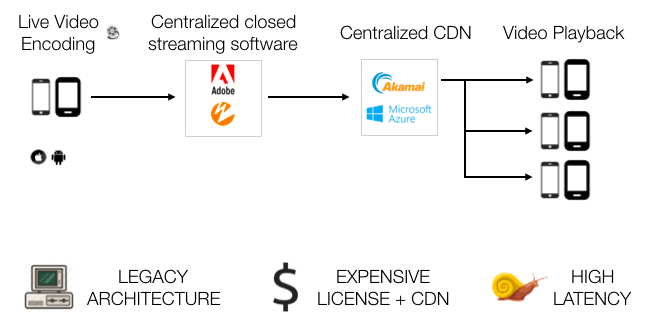
\includegraphics[width=1.0\textwidth]{problem-architecture}
  \caption{Current closed, centralized, expensive, censorable live streaming system}
  \label{image:problem-architecture}
\end{figure}

Figure \ref{image:problem-architecture} shows the state of current live streaming system. There are 4 components to a live streaming system. They are explained below.
\subsubsection{Broadcasting Software}
A proprieteary mobile video encoding software is used. The primary purpose of this software is to capture video frames and audio, from mobile, desktop, or stand alone cameras. The software encode the captured video and audio frames into a video standard, and a closed/proprietary video streaming protocol and is published to Streaming software.

\subsubsection{Broadcasting Server Software}
Incumbent software that solves this problem are Wowza\footnote{https://www.wowza.com/products} and Adobe\footnote{https://www.adobe.com/products/catalog.html}. The Broadcasting software receives the encoded live streams and generates small fragments of video files that are then published to a Content Delivery Network.

\subsubsection{Centralized Content Delivery Network}
The Broadcasting Server Software publishes the generated video fragment files to Content Delivery Network such as Amazon Cloudfront \footnote{https://aws.amazon.com/cloudfront/} or Microsoft Azure \footnote{https://azure.microsoft.com/en-us/services/media-services/}

\subsubsection{Video Player}
This is the final step in live video streaming. Media/Video/Audio clients for platforms: mobile, desktop, play out the video files from the content delivery networks.


These are the problems with current live streaming system:
\begin{itemize}
  \item{Centralized points of failures: Backend streaming software, relying on content delivery networks}
  \item{Proprietary and closed source software}
  \item{Prone to censorship as easy to control/shutdown the service}
  \item{Expensive licensing fees}
\end{itemize}

\subsection{Hootcoin Solution / Hoot Network Solution/ Hoot Solution}
 \fxerror{fix name for everything Hootcoin network, Hootcoin Token, Hootcoin protocol team, Hootcoin Foundation need right names for all and replace all }.

\begin{figure}[h!]
  \centering
  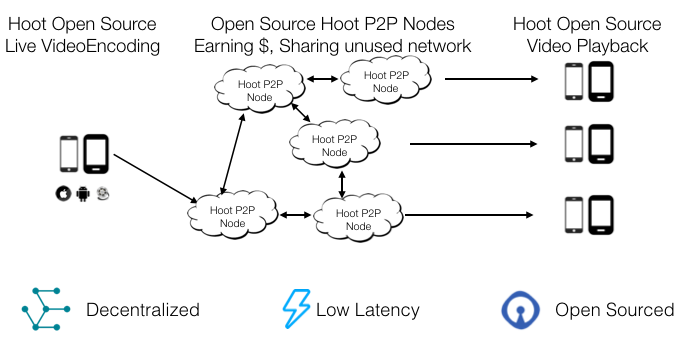
\includegraphics[width=1.0\textwidth]{hoot-solution}
  \caption{Open Source, decentralized, censorship resistant Hoot live streaming system}
  \label{image:hoot-solution}
\end{figure}


Figure \ref{image:problem-architecture} is the proposed live streaming system. They are explained below.
\subsubsection{Hoot Open Source Broadcasting Software}
Hoot Open Source Broadcasting captures video frames and audio. All major platforms: iOS, Android, Mac, Windows, Linux will be supported. The captured video frames and audio data are encoded to widely accepeted open video and audio formats: H.264 and AAC. The encoded H.264 and AAC audio is published to the Hoot Network with Real Time Hoot Protocol.

\subsubsection{Hoot P2P Node}
Miners in the Hoot P2P node will run Hootcoin software sharing unused bandwidth and earning Hootcoins for doing so. This is a highly resilient fault tolerant network, and miners will be able to join or leave the network anytime. The Hoot P2P Node replaces the need for a broadcasting server software and expensive content delivery network.

\subsubsection{Hoot Open Source Video player}
Hoot Open Source Video player plays the live stream in realtime. All major platforms: iOS, Android, Mac, Windows, Linux will be supported.

\subsubsection{Archived videos}
Broadcasted video are also continously archived, and will be stored in decentralized file system IPFS \footnote{https://ipfs.io/}

Hoot live stream protocl make the live streaming faster, safer, and more open by

\begin{itemize}
  \item{No centralized points of failures - byzantine fault tolerant p2p network}
  \item{Highly resilient fault tolerant network with peer to peer nodes}
  \item{Censorship resistant as there are no centralized points of control}
  \item{core peer to peer and networking software is open source}
\end{itemize}

\section{What makes Hoot special}
When compared to other products on the market, Hoot has several defensible advantages:
\begin{itemize}
\item[-]Optimized for 2G/3G networks around the world, low CPU and GPU usage, saves battery and bandwidth consumption
\item[-]Next-gen live-streaming product that enables self-serve streaming from mobile
\item[-]Allows to interleave background music in a seamless manner
\item[-]Break through patent-pending technology architected from the
  ground up requiring no licensing fees
\item[-]Hoot offers instant archival of live-stream videos making it unnecessary to upload files again at the end of livestream
\item[-]Modular architecture allows building tor/vpn modules inorder
  to enable uncensorable livestreaming to promote free speech
\end{itemize}


\section{Traction \& Usage}
A mobile consumer application is currently live on the iOS AppStore and Google Playstore. Hoot has received streams from 

\fxerror*{put right numbers}

Tables \ref{table:1} and \ref{table:2} show the usage statistics.

\setlength{\arrayrulewidth}{.7mm}
\setlength{\tabcolsep}{18pt}
\renewcommand{\arraystretch}{2.0} 
% \newcolumntype{s}{>{\columncolor[HTML]{AAACED}} p{3cm}}
% \arrayrulecolor[HTML]{DB5800}
 


\begin{table}[!htb]
\centering
\begin{tabular}{ |c|c| }
\hline
\rowcolor{lightgray} \multicolumn{2}{|c|}{User Statistics} \\
% \hline
% Metric Name & Metric Value  \\
\hline
Monthly Active Users (MAU) & 214,769 \\
% \rowcolor{gray}
Total Users & 3,000,000  \\
\hline
\end{tabular}
\caption{User Statistics}
\label{table:1}
\end{table}

\begin{table}[!htb]
\centering
\begin{tabular}{ |c|c| }
\hline
\rowcolor{lightgray} \multicolumn{2}{|c|}{Live Video Streaming Statistics} \\
% \hline
% Metric Name & Metric Value  \\
\hline
Number of Videos & 48,207 \\
Average Viewers per stream & 155 \\
Average Stream Duration & 4 minutes 35 seconds \\
Total Time Watched & 37k days or 100 years \\
% \rowcolor{gray}
\hline
\end{tabular}
\caption{Live Video Streaming Statistics}
\label{table:2}
\end{table}



\section{Low Latency Streaming Technology}
\fxerror{maybe not needed}
How hoot powers low latency streaming.

\section{Hoot Architecture}

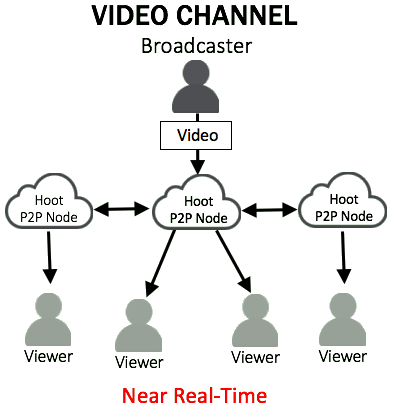
\includegraphics[scale=0.5]{static/hoot-video-architecture-channel-trans}

\subsection{Broadcast Side - mobile iOS client}
The protocol for realtime livestreaming video is called Real-Time Satoshi Streaming Protocol[\textbf{RTSSP}].
Video frames are captured at a resolution of 540x960 to 720x1280 based on network connectivity. Audio stream is captured using the built in iOS device microphone at a sampling rate of 44.1 KHz. Optionally, real time filters (Black and White, Glow, Fisheye, Sepia) can be applied to captured video frames in real-time. Video and audio are encoded using the native hardware H.264(H.265 in android) and AAC encoders, respectively. The video frames are encoded using a VBR algorithm with a maximum bitrate of 1 Mbps, this can be increased for usecases such as VR streaming. Audio stream is encoded in AAC format with a bitrate of 128 Kbps. The H.264 + AAC stream is encoded into an RTSSP stream and is transmitted to Hoot RTSSP server.

\subsection{Broadcast Side — Desktop Mac client}
Video frames are captured at native screen resolution, and audio stream is captured using the built in microphone at a sampling rate of 44.1 KHz. Hoot native cocoa Mac app written in Objective-C supports capturing FaceTime, Screenshare, and a combination of FaceTime and Screenshare. Video frames and audio stream are encoded using the native H.264 and AAC encoders, respectively. The video frames are encoded with a VBR algorithm. Audio stream is encoded in AAC format with a bitrate of 128 Kbps. The H.264 + AAC stream is encoded into an RTSSP stream and is transmitted to the open source RTSSP server.

\subsection{Viewer Side mobile iOS/Android client }
 Hoot open source Native mobile media player decodes RTSSP + H.264 and AAC data to make the live broadcast available to viewer in real-time. The HLS (HTTP Live Streaming) stream that is made available can be played using the iOS/Android Native media players, when the Hoot RTSSP player or app is not available.

\subsection{Viewer Side Mac/ Destkop PC client} 
The RTSSP stream is played using Adobe Flash technology supported by modern browsers. The HLS stream can be played using HTML5 player available in modern browsers.

\subsection{Server Side Peer-to-Peer decentralized Technology}
Similar to Bitcoin blockchain technology, any node can join or leave the Hoot network at anytime. Each node runs a realtime broadcasting server.
The GPUCoin network has several RTSSP servers that serve to bootstrap the Network. We use commodity servers with modern processors and with 1 Gbps duplex ethernet; specialized servers are not needed. The hoot server generates two variants of streams: a RTSSP stream and a HLS stream in order to make them accessible in browsers across Windows, Mac OS, Linux and Android platforms. A server with 1 Gbps duplex ethernet can support up to a total of 1000 viewers. A stream is replicated horizontally across multiple servers (without additional latency) to stream to virtually an unlimited number of simultaneous viewers. 

Streamed videos are instantly archived [\emph{H.264+AAC, mp4 container}] in the cloud for later viewing. The archived videos are indexed (scrubbable and quick to scan). We have access to datacenters in the following geographically distributed locations through RTSSP servers to provide the least latency to viewers globally: Amsterdam Netherlands, Frankfurt Germany, Hong Kong, London UK, Melbourne Australia, Queretaro Mexico, Milan Italy, Montreal Canada, Toronto Canada, Paris France, Singapore, Sydney Australia, Tokyo Japan, Dallas TX, Houston TX, San Jose CA, Seattle WA, Washington DC. 
% \sout{}
Streams are replicated and pulled to the closest node to the viewers location, i.e., a viewer in Tokyo Japan viewing a stream from Washington DC would be connected to a replicated stream on the Tokyo Japan hoot node in order to reduce latency.



\section{Security}
The live connection is encrypted using AES\_256\_CBC, with HMAC-SHA1 for message authentication and DHE\_RSA as the key exchange mechanism. Every Hoot opensource player connection is authenticated.
An authorization key is needed to view a private Hoot video stream. Signup, interactions, HLS streams and archived static content are end-to-end HTTPS  SSL encrypted to ensure strong security.    

\subsection{Anonymity and privacy over VPN and Tor}
Anonymity and privacy are key to enable free speech, and this matters
more in countries where free speech continues to be an ongoing human rights
issue. In combination with blockchain technology, the network is
designed to route video streams and meta data over VPN and optionally
Tor network to avoid censorship and promote free speech.

\section{Hoot Monetizing Engine}
Hoot tokens based on cryptocurrency technology power the Hoot
marketplace and economy. Hoot miners earn hoot tokens running their own open source
de-centralized hoot nodes utilizing the unused networking bandwidth
and compute capacity they may have. In countries where censorship is an issue they
may run de-centralized hoot nodes with Tor/VPN modules enabled so they can
support free speech through hoot
live-streaming. Hoot tokens can also be used by viewers to support their favorite artists,
musicians and gamers. They may send hoot tokens to the
streamers they love watching and for events that they want to
support. Streamers can also earn hoot tokens by enabling subscriptions in order to have a
dependable source of recurring revenue. This enables them to make a
living off their fan base from the comfort of where they are without
having to spend for event space and the complicated offline
co-ordinating schemes needed to assemble all their fan base for their events.

\sout{For micropayments, artists can safely accept the hootcoin payment immediately.  The size of the payment is too small for the effort to steal it. Micropayments are almost always for intellectual property, where there's no physical loss to the merchant. }

 Hoot network will also build marketing and sales tool to help
streamers and gamers market their 
events and build a paid subscriber base using email lists and sms lists among other social media
channels. 
Musicians can also use the album selling tools to list and sell
their albums, singles and release music videos. They can
choose to exchange their hoot tokens earned for crypto-currencies or fiat currencies.
 Streamers can also use hoot tokens to
purchase advertising space to feature events or utilize the marketing and sales
tools to drive more viewers to their
streaming events such as an album launch, book launch, movie launch or
e-sports gaming event. Hoot miners, streamers and viewers can also load Hoot
tokens on to their respective accounts using crypto-currencies such as Bitcoin,
Ethereum, Litecoin, Monero, Zcash and fiat currencies such as USD, EUR among others.

\subsection{Performant Augmented Reality ads with measurable ROI }
Video Ads have been priced historically based on CPM for impressions as it has been nearly impossible to know how much of these video ads lead to a product sale/conversion or if they even positively affect the customer ROI. Viewers do not know what action to take and how to take the said action leaving them to figure out how to follow up on the video ad they just saw, leading to a lot of drop off and lack of performance of these video ads. Hence It’s not easy  to measure effectiveness and performance of the video ads historically.

Using interactive \textbf{Hoot AR} augmented reality  ads with clear calls to Actions such as a buy button or rent button below the interactive Hoot AR ad, sales can be generated right then and there, after the viewer interacts with the Hoot AR ad. We will be able to charge based on sales generated from the AR interaction i.e., referrals and instead of charging based on CPM or impressions we can price based on  cost per referral(\textbf{CPR}). The CPR price becomes the signal that drives the continuous auction engine that powers the Hoot ad marketplace. By bringing about an innovative CPR based business model to video ads using Augmented reality \emph{call-to-actions} we bring the effectiveness of Google AdWords to video ads that only used to perform as well as banner ads before. Hence Hoot AR ads, improves the effectiveness of plain video ads, leading to a quantum improvement in video adspend ROI much like AdWords improved the ROI of web based banner ads.

\section{Hoot video platform, plugins and video AppStore to support machine learning,
  augmented reality, VR and video v-apps}
We are quite excited by ARKit that is going to be available in the
upcoming version of iOS11 and believe that it is going to usher a
golden era of augmenting reality in video-streaming. With Tensorflow,
Caffe, Keras, Theano, TensorFlow Object Detection API, GCP cloud
video intelligence api and Azure video machine-learning apis there is going to be a
big wave of machine learning video content-analysis applications,
makes videos searchable, and discoverable. You can now search every
moment of every video file in your catalog and find every occurrence
as well as its significance. Hoot video primitives via API/SDK will allow developers to extract
actionable insights from video files without requiring any machine
learning or computer vision knowledge. 

 We want to enable a
thriving ecosystem by building a video appstore and provide a scalable
platform for video developers around the world. By providing an
extensible plugin architecture, we will allow developers to build
plugins on the Hoot video architecture. Filters, face-detection and face-swapping
are some early augmented reality ideas that will be explored. \sout{Some interesting
machine-learning and ai ideas are Label Detection(Detect entities
within the video, such as "dog", "flower" or "car"), Shot Change
Detection(Detect scene changes within the video),
Regionalization(automagically specify a region where processing will
take place), automated subtitle detection, Home and office security and others yet to be discovered.} By enabling a platform
play with easily extensible and scriptable plugins, and video appstore
for AR and ML/AI v-apps, we will accelerate the golden age of
intelligent live video.


\subsection{Un-censorable P2P identity and reputation blockchain}
Since there is an economy of trading in the marketplace of the Hoot network, having a Peer to peer
identity and reputation database to enable seamless, non-custodial
de-centralized, trust-free interactions becomes essential. Feedback and reviews as well as point scoring out of a maximum of 5 and minimum of 1 for quality of interactions factor into an agents reputation trust score. The trust score of each agent is hashed into the blockchain using their public gpg key and hashed username so as to make them Un-censorable. Trust score and reviews may only be added to the database and nothing can ever be removed making this the trust reputation blockchain. \textbf{Merkle trees},an efficient verifiable datastructure, are used to ensure the reputation db is usable by downloading the relevant sub-tree for a particular user hash even as the reputation blockchain grows very large in size as the network grows exponentially.

\subsection{Multi-sig escrow wallets}
Hoot tokens are first sent to a multi-sig escrow wallet, that is controlled by the buyer/viewer, seller/streamer and an
independent third-party escrow. Any
two out of the three parties need to sign in order for the transaction to be
completed. Also the number of times the buyer or seller necessitates
escrow agents to mediate a dispute and the time to complete a
transaction will factor into the reputation of the buyer and
seller. Any trusted agent with a high enough reputation score can
register to be an independent third party escrow agent. Escrow agents
also earn feedback and trust which are hashed and stored in the
blockchain using their public gpg key and hashed username so it
becomes un-censorable.


\subsection{Auction to find optimal price}
To bootstrap the network, Hoot network will run Vickrey auctions to find the best service to run on the miners computer that has excess capacity. A \emph{Vickrey auction} is one in which the winner pays the second-highest price, not the price they themselves bid, which has been effectively used by Google adsense and adwords.
Hoot can instantiate any auction protocol, if they find a suitable auction protocol that is superior to Vickrey. Its seed protocol specifies a procedure for stakeholders to approve amendments to the auction protocol,
\emph{including} amendments to the auction amendment procedure
itself. Upgrades to Hoot auction protocol are staged through a testing
environment to allow stake-holders and token-holders to recall potentially inferior
amendments, that lead to sub-optimal pricing for network
stakeholders. 

Since the hoot network can also be used for other tasks than streaming live video, the network can be extended to run any computing task such as computer graphics, business applications, machine learning, crytography, malware prevention analysis, science and services, making the Hoot network a Uber for computers, enabling miners to rent their unused CPU/GPU cycles and get paid in Hoot cryptocurrency. Hence the Hoot de-centralized network powers true cloud computing.

\subsection{Cryptocurrency And Issuance}

The Hootcoin network includes its own built-in cryptocurrency, Hootcoins, which serves the dual purpose of providing a primary liquidity layer to allow for efficient exchange between various types of digital assets and, more importantly, of providing a mechanism for paying transaction fees.

The issuance model will be as follows:

\begin{itemize}

\item Hootcoins will be released in a cryptocurrency sale at the price of 1000-2000 Hootcoins per BTC, a mechanism intended to fund the Hoot organization and pay for development that has been used with success by other platforms such as Mastercoin, Filecoin, Ethereum, Tezos and NXT. Earlier buyers will benefit from larger discounts. The BTC, ETH, XMR, and LTC received from the sale will be used entirely to pay salaries and bounties to developers and invested into various for-profit and non-profit projects in the Hoot cryptocurrency ecosystem.

\end{itemize}

\subsection{Hoot carbon footprint, mining, scarcity and profitability}
Bitcoin has made cryptocurrencies popular and brought it to the mainstream, but it has a dark side, its ever increasing carbon footprint. In late 2013, 8.25 megatonnes (8,250,000 tonnes) of CO$_2$ per year
was estimated to be the carbon footprint of Bitcoin per year\footnote{https://pando.com/2013/12/16/bitcoin-has-a-dark-side-its-carbon-footprint/}. These
computers are consuming so much electricity that it’s already
unprofitable to mine in some regions of the world. Since excess
bandwidth and compute capacity is utilized towards streaming,
encoding, object recognition
and security of video and audio streams the resources otherwise would
be utilized are profitably used.  Since Hoot tokens are fairly distributed to miners corresponding to their compute and bandwidth availability irrespective of how much CPU they control, the Hoot carbon footprint will be exponentially lower than the Bitcoin network which depends on continuously increasing complexity of the hashing required for mining. Since hoot tokens can only be mined or acquired from the platform, they will tend to be a scarce token.

\section{The Foundation and Governance} % (fold)
\label{sec:the_foundation_and_governance}
As a company limited by guarantee established in Switzerland, the Hootcoin Foundation's primary objective is to promote the real world application of the Hoot Decentralized Open Live Streaming platform. It also aims to initially develop the Hootcoin platform and advocate governance and transparency for the platform. The Hootcoin Foundation will establish an association consisting of members of the Hootcoin ecosystem, which will be empowered to determine the direction of functionality and improvement to the Hoot Live Streaming platform and associated ecosystem.
% section the_foundation_and_governance (end)

\subsection{The dispute resolution process} % (fold)
\label{sub:the_dispute_resolution_process}
The Hootcoin Foundation will specify a dispute resolution process, utilizing an internationally accepted dispute resolution system. A rotating board of dispute referees will monitor disputes through the resolution process, and oversee collateral release to plaintiffs. Note that this board of dispute referees is not the dispute resolution process specifically; rather it is the mechanism through which dispute resolutions can be enacted through the release of collateral on the blockchain.


\subsection{Hootcoin Token sales} % (fold)
\label{sub:hoot_token_sales}
The Hootcoin Foundation will fund the development of the Hoot Live Stream Platform discussed in this paper through the issuance of Hootcoin tokens. These tokens will run natively on the Ethereum blockchain and will be offered to backers of the Hoot Live Stream  project via a token sale. The token sale will be launched on or about the 22nd September 2017. A second token sale will take place once the initial prototype has been developed and tested to fund its deployment. For more information on the Hoot token, see \_\_\_ \fxerror{add correct section}.

\subsection{Token Allocation and Distribution} % (fold)
\label{sub:token_allocation_and_distribution}
 The supply of Hootcoin is limited to the number of one hundred million (100,000,000) in total (including those available for sale during the Token Sale) and will be generated upon the launch ("Token Launch".)

 The tokens will be distributed in the following manner:
80\% (30/30/20) of the tokens will be eventually allocated amongst the community; the remaining 20\% will be allocated to the Hootcoin Foundation initiator, early backers, and the Hootcoin protocol network development team.


\begin{table}[!htb]
\centering
\begin{tabular}{ |p{2.8cm}|p{2.5cm}|p{5cm}|}
\hline
\rowcolor{lightgray} \multicolumn{3}{|c|}{Hootcoin Token Distribution Model} \\
\hline
Channels & Percentage & Lock up Period  \\
\hline
30,000,000 HOOT  Hootcoin Token Sale (HTS) & 30\% & Token Sale - Launch 22nd September 2017. The initial funding will be used to develop a working prototype, financial setup, legal fees and promotion.
 \\
 \hline
30,000,000 HOOT Additional Hootcoin Token Sale (AHTS) & 30\% & Additional Hootcoin Token Sale. On the release of a successful prototype, a second token sale will be launched to fund the full production ready launch and development of all relevant technology and organization matters.
\\
\hline
20,000,000 HOOT Retained by the Foundation as Treasury & 20\% & 100\% of which locked for 24 months.Strategic Planning, Project Support, Token Swap, Emergency Fund, Development \& Legal Fees - These will be subject to a 2- year lock-up. Subsequent to the lock-up, these will be used for various development and operation costs of Hoot Platform over 2 further years.
\\
\hline
20,000,000 HOOTcoin Advisors, Directors and Early Backers & 20\% & 70\% of which locked for 12 months. 30\% of which is locked up for 24 months. Distributed to the directors, advisors, and early backers of the
 project.
\\
 \hline
\end{tabular}
\caption{Hootcoin Token Distribution Model}
\label{table:hoot_token_distribution_model}
\end{table}

\fxerror{clean up table, better formatting/fonts}

\subsection{Restriction on the use of the funds} % (fold)
\label{sub:restriction_on_the_use_of_the_funds}
To remain in line with the spirit of the project’s open and transparent philosophy, all funds shall be tracked and reported according to the Foundation’s guidelines. A custodian will monitor the usage of the digital tokens and share it with the community periodically.

\begin{enumerate}
  \item Financial planning and reporting
  \begin{itemize}
    \item The Hootcoin Foundation shall develop financial planning and review financial
performance of the previous quarter.
  \end{itemize}

  \item Digital tokens management
    \begin{itemize}
    \item The digital tokens belonging to the Foundation shall be managed by authorized personnel. The security of digital tokens is ensured by multi signature technology.
  \end{itemize}

  \item Digital wallet protocol
    \begin{itemize}
    \item The Foundation’s digital wallet shall be protected by a multiple signature technology mechanism.
  \end{itemize}

  \item Disclosure
    \begin{itemize}
    \item On a regular basis, the Foundation shall disclose on the topics regarding community matters, including status of development, operations, and the usage of tokens, as well as whether the Foundation operates in accordance with the governance policy.
  \end{itemize}
\end{enumerate}


\section{The Hootcoin Token}
The Hootcoin Token (HOOT) is a native Ethereum divisible digital token with up to 18 decimal places. The total number of OAX tokens to be issued is 100,000,000. For details of the distribution of these tokens, see Section \ref{sub:token_allocation_and_distribution} \nameref{sub:token_allocation_and_distribution}.

\subsection{Uses of Hootcoin Token} % (fold)
\label{sub:uses_of_hoot_token}
Hootcoin token can be used for using the platform.
\fxerror{need to add economics of bandwidth sharing}

% subsection uses_of_hoot_token (end)
% subsection subsection_name (end)

\section{Hootcoin Development Timeline}
The Hoot consumer mobile app which uses Facebook or Twitter to authenticate is already live in the iTunes AppStore\footnote{Hoot live on iOS AppStore https://appsto.re/us/40RS-.i} and Google Android Play Store\footnote{Hoot Live on Google Playstore https://play.google.com/store/apps/details?id=com.onhoot.android}.
A light weight performant native  mac app is live on
the website \footnote{Download link for Hoot Live on Mac Desktop https://onhoot.com/mac}. The mac app can be used to screen-share meetings, conferences and webinars. It can also be used
to livestream desktop games such as Minecraft, league of legends,
world of warcraft and others.

A native enterprise version that uses Slack for authentication of
internal private teams is already live.
 This requires quite a bit of work to integrate with the slack teams api and also in order  ensure security for private teams. Following platforms are supported
\begin{itemize}

\item[-]iOS app for slack private teams \footnote{ iOS private Hoot business client for slack teams http://hootvideo.com/business}
\item[-]Hoot Mac desktop app for slack private teams \footnote{Desktop Hoot client for Slack teams http://hootvideo.com/macbusiness}
\item[-]All modern browsers. \footnote{Slack based private team build of Hoot https://hootvideo.com}
\end{itemize}

Web browser end points are live on line as well
\footnote{Hoot live link on Web browswer https://onhoot.com}. The minimum requirements are any modern
browser such as Safari, Mozilla Firefox, Microsoft Internet Explorer
or Google Chrome which fallback to HTML5 HLS video format for playback
of the live-streams.


\subsection{Tor and VPN to enable uncensorable live-streaming }
Tor modules to live-stream video over the onion routed tor network needs
to be built. Integration with VPN needs to be built in order to evade censorship. This would enable true zero knowledge live-streams and computing in
countries where censorships and free speech continue to be ongoing
human rights issues.

The underlying hoot technology may also be used to build an open
source low cost security and surveillance alternative to closed systems
such as Nest.

\subsection{Focus on Performance}
We have a strong focus on performance and highly performant applications while still maintaining smaller binary sizes and  code integrity. The hoot iOS app is under 10MB, the latency is under a second plus the network latency. This leads to a superior user experience and efficient usage of unused compute.

\section{Uber for Computers creating IPCN - Interplatenary compute network}
Hootcoin network is a dense Byzantine fault tolerant peer-to-peer network - creating the IPCN - Interplatenary compute network.
Hootcoin Network is based on a complex architecture revolving around P2P, Blockchain, Smart Contracts, State Channels. Hootcoin network protocol will enable the creation of completely decentralized compute network, powered by decentralized cryptocurrneyc micro payments. This leads to Uber for computers helping create the worlds first IPCN an interplatenary compute network. We will create a platform to create new compute primitives using any turing compute programming language. We will use container technologies such as  docker and kubernetes to efficiently distribute and use excess unused compute. The compute results of the network are verifiable using cryptographic and mathematical properties of the cryptographic design. The IPCN takes advantage of the coming cambrian explosion of computing, cryptocurrencies and CPU/GPU miners.


\section{Conclusion}
Bet on the future with Hoot live streaming protocol.


% \renewcommand{\lstlistingname}{Appendix}
% \begin{lstlisting}[caption={Digital Fingerprint},captionpos=b, language=java,numbers=none]

% {
%     "$schema": "digital_fingerprint",
%     "definitions": {},
%     "id": "https://hootvideo.com/whitepaper",
%     "properties": {
%         "compressedContent": {
%             "id": "/properties/compressedContent",
%             "items": {
%                 "id": "/properties/compressedContent/items",
%                 "type": "integer"
%             },
%             "type": "array"
%         },
%         "link": {
%             "id": "/properties/link",
%             "type": "string"
%         },
%         "name": {
%             "id": "/properties/name",
%             "type": "string"
%         },
%         "publishDate": {
%             "id": "/properties/publishDate",
%             "type": "string"
%         }
%     },
%     "type": "object"
% }

% \end{lstlisting}
\newpage
\listoffigures
\newpage 
\listoftables
\newpage 
\bibliographystyle{plain}
\end{document}

\end{lstlisting}

\bibliographystyle{plain}
\end{document}

